\chapter{Exploratory Analysis}
\label{chap: exploratory}
First part of the analysis is to explore the different attributes in the data, in order to detect possible patterns or correlations. The exploratory analysis is also used to get an understanding of data and its behaviour. Hence, this chapter is about visualizing the different attributes focusing on their influence on the heat consumption. As the heat in each house is turned off in the summer period, data is segmented such that the summer period is excluded from the data used for modelling. \\

\section{Examination of the Heat Consumption}
\noindent To get an overview of the heat consumption for each house, the daily average heat consumption for each house is investigated. \cref{fig: daily_cons} shows the daily average consumption for all the houses and the daily consumption of two houses - one that follows the trend and one that deviates. These two houses are chosen to be visualised throughout the report and their specifications are presented in Section 3.1.2. It can be seen that the slopes around the summer months are close to 0. As mentioned, the data in focus in this project is where the heat is turned on, hence the period where the heat consumption is close to 0 needs to be removed. Exactly how this is done will be explained and discussed in the data segmentation section. All three plots show some unusual high data points around April 2018. This can be due to the fact that is was snowing in Denmark at that time which is supported by the article found in \cite{vejr2018}. \\
\begin{figure}
    \centering
    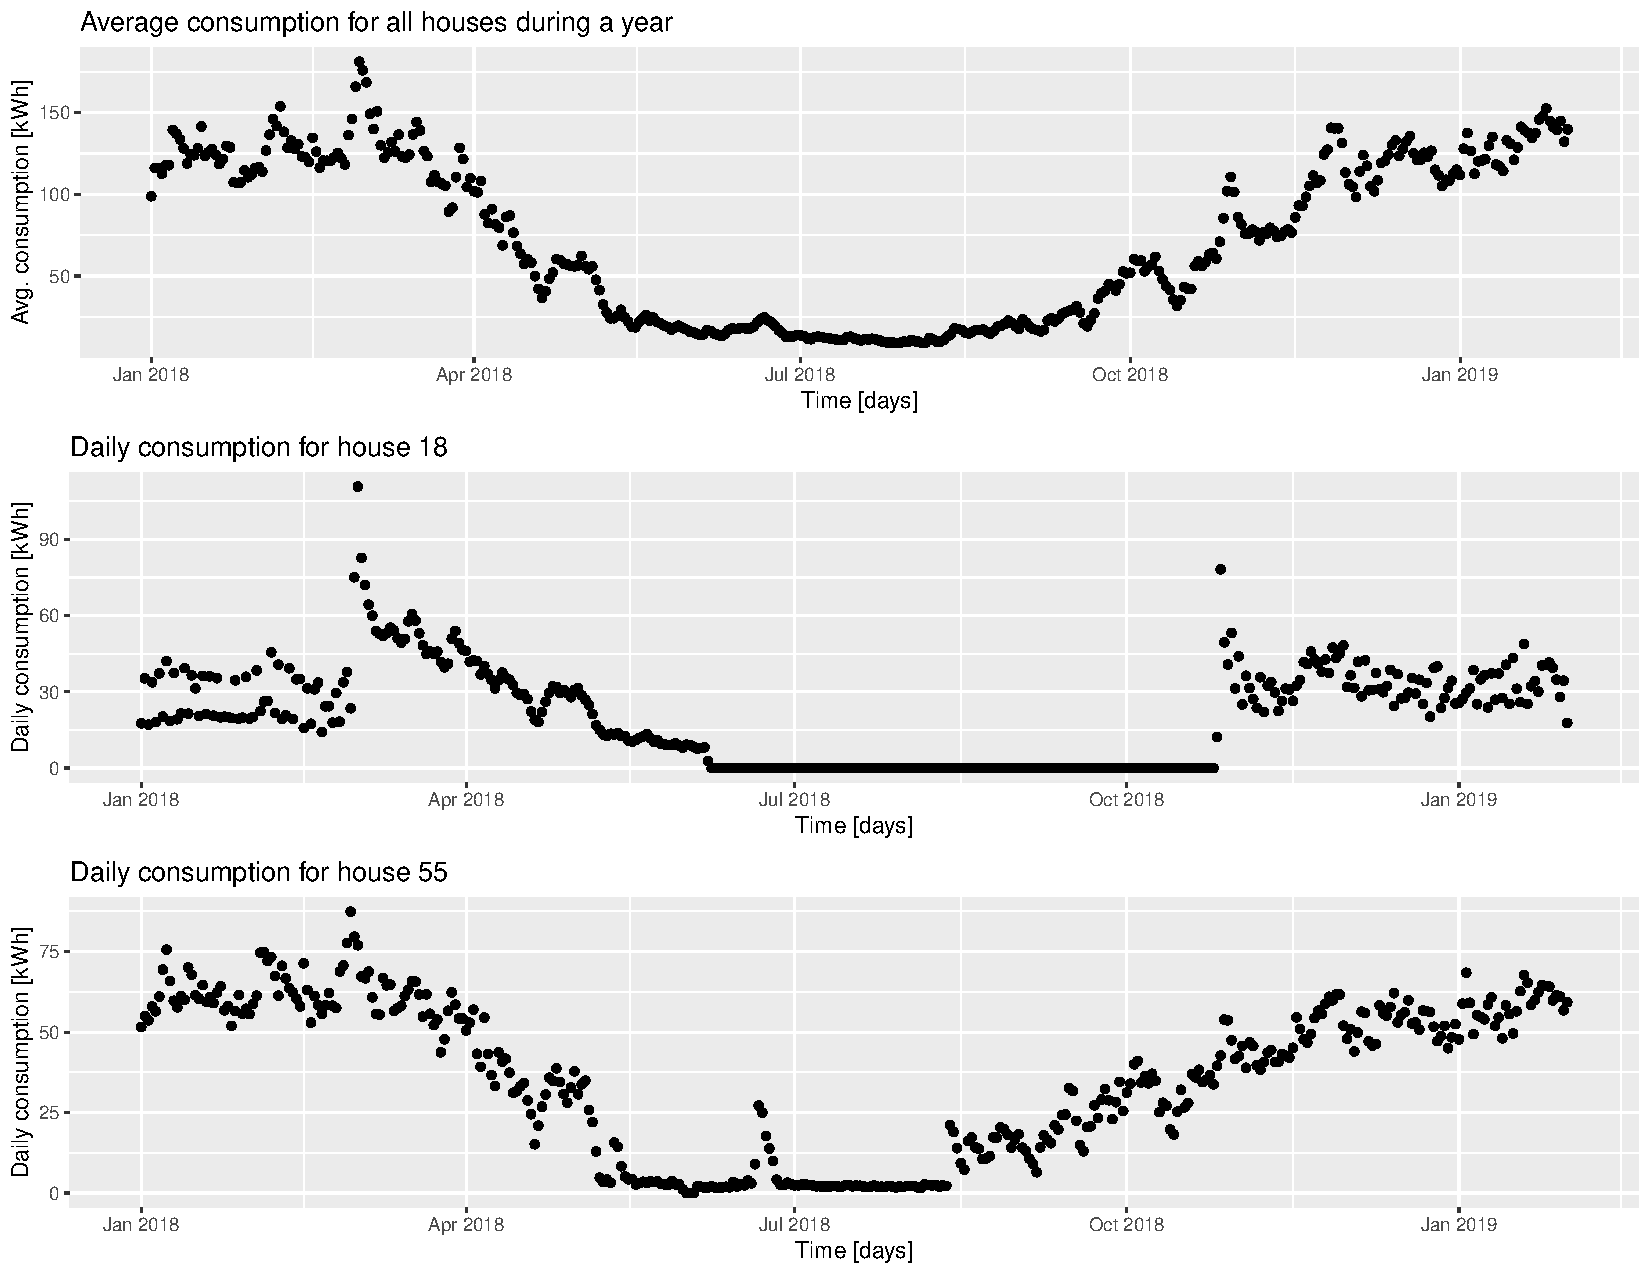
\includegraphics[width=1.\textwidth]{../../../figures/daily_cons.pdf}
    \caption{Daily consumption during a year (2018). The top plot shows the average consumption for all the houses. The plot in the middle shows an example of a house that deviates from the trend and the last plot shows a house that follows the trend}
    \label{fig: daily_cons}
\end{figure}

\noindent The remaining attributes from the house data is examined through a scatterplot shown in \cref{fig: housepairs} and \cref{fig: house_attri}, in order to find possible linear relationships with the consumption. There are clear linear relationships between the consumption and the flow, the volume, the cooling degree and the temperature going in respectively. It is expected that the consumption depends linearly on the volume and cooling degree, cf. the main equation given in \cref{eq: Q_heat}. The relationships between consumption and the flow and volume are quite similar which is in line with the description of the two attributes given in \cref{tab: housedata}. It is also seen that the temperature of the water coming out of the system depends on how much is used. So if the return water is quite hot, 
the house has not fully utilized the heat for the heat consumption. 
\begin{figure}
    \centering
    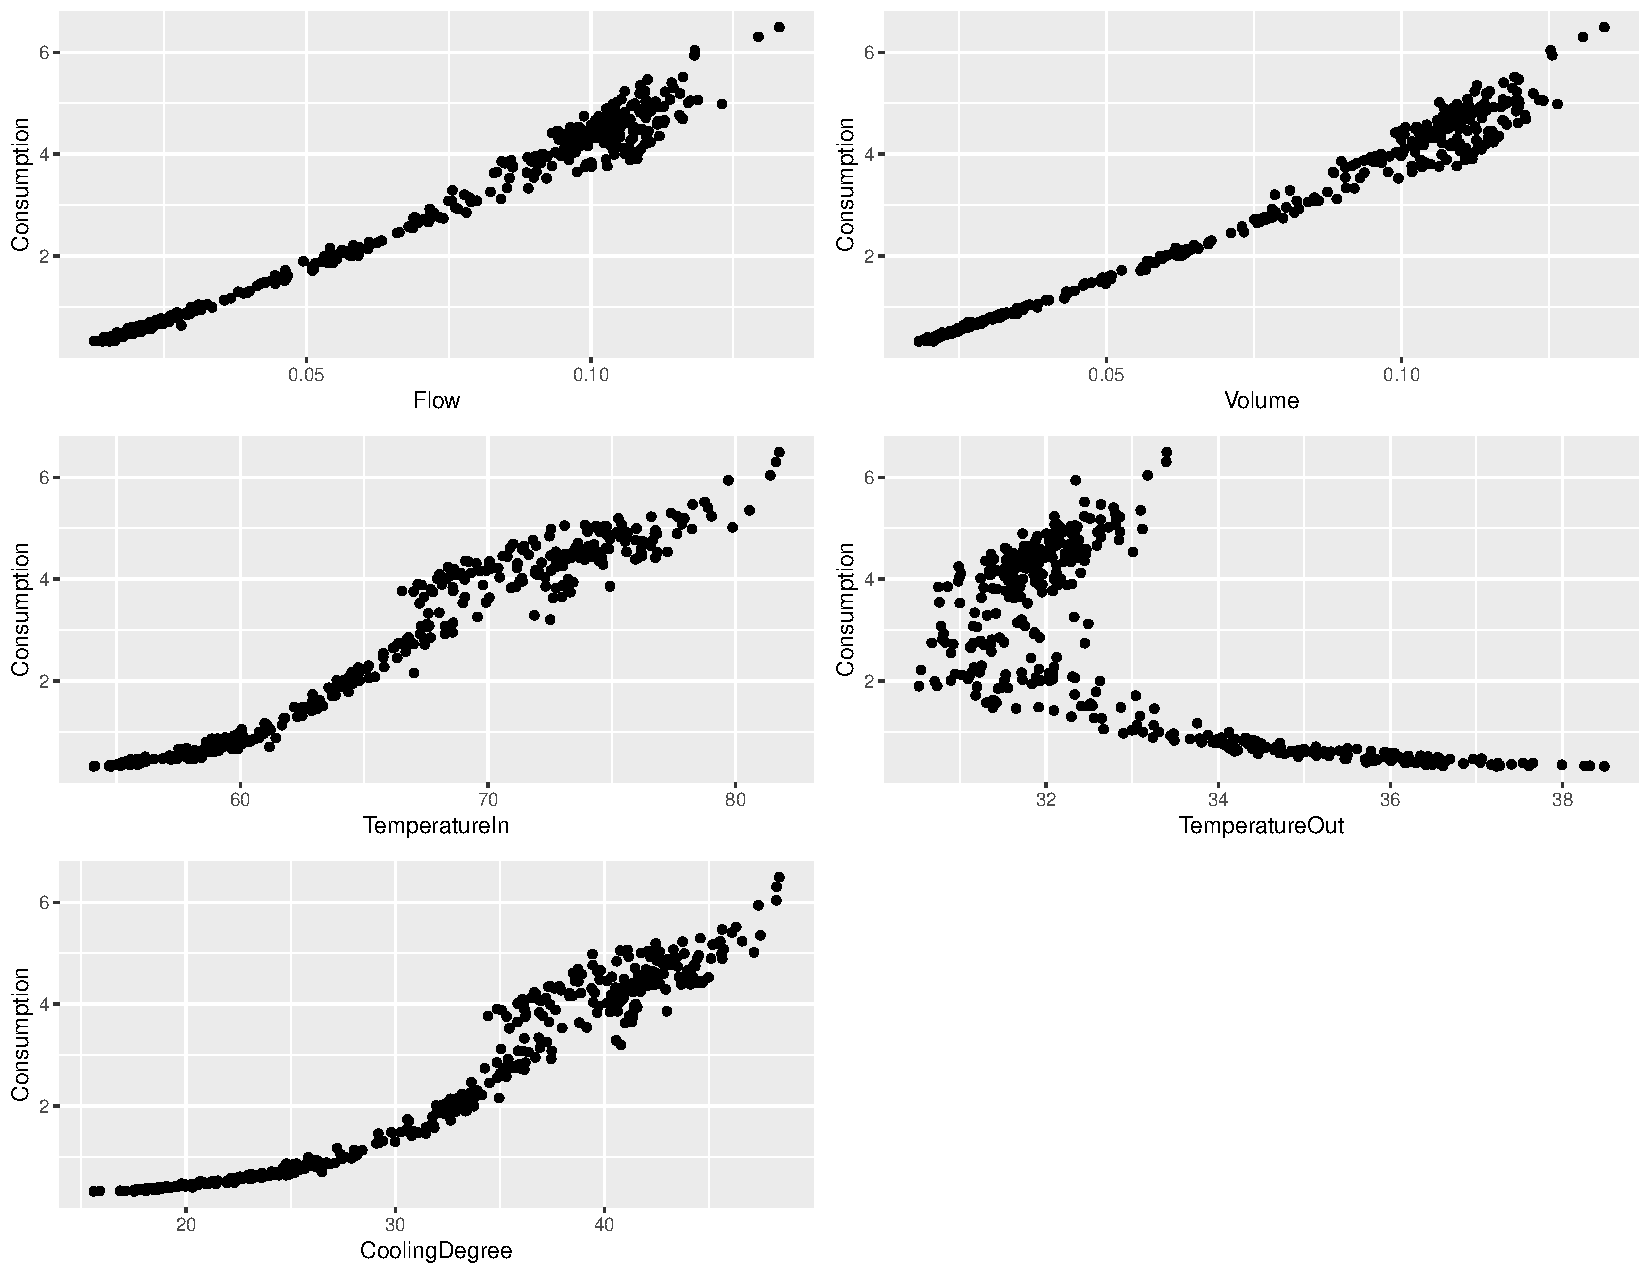
\includegraphics[width=1.\textwidth]{../../../figures/housepairs.pdf}
    \caption{Scatterplots of the average consumption for all houses and relevant house attributes. Each point represents a day. There are clear linearly dependencies between \texttt{Consumption} and e.g. \texttt{Flow}} 
    \label{fig: housepairs}
\end{figure}

%\noindent Figure \ref{fig: house_attri} clearly shows that the consumption is close to 0 in the summer period.  
%\textcolor{red}{Pairs af gennemsnitlig house data - vi ser en masse sammenhænge mellem de forskellige attributer. Vi kan se at CoolingDegree skal være over 25, før at varmeforbruget stiger.}
%\textcolor{red}{CoolingDegree begynder at stige et stykke tid før flowet stiger, hvilket hænger godt sammen med at når man fx tænder en radiator så stiger CoolingDegree. De efterfølgende radiatorer man tænder øger volumnet.} \\

%\textcolor{blue}{\noindent It is already known that there is a dependency between the heat consumption and the time of the year. During the summer period there is almost no consumption. The consumption in this period is probably mostly tap water. The next important thing is the relation between temperature and consumption. High temperatures tend to imply a higher consumption. And the reason why the consumption depends so clearly on the time of year can be assumed to that certain periods have similar temperature levels. It can also be seen that there is a correlation between dewpoint and consumption. This can be due to the correlation between dewpoint and temperature.}

\subsection{Weather data}
The weather data is also examined through scatterplots given in \cref{fig: weatherpairs} and \cref{fig: weather_cons} in order to detect dependencies between the average consumption of the houses and the weather attributes. It is already known that the outside temperature has a significant influence on the consumption which is in line with the linearly relationship between the temperature and the consumption in \cref{fig: weatherpairs}. Furthermore, consumption is approximately influenced by the dew point which is probably explained by the linear relationship between \texttt{Temperature} and \texttt{DewPoint} illustrated in \cref{fig: weather_cons}. The scatterplots show that the consumption overall is independent of the attributes \texttt{WindSpeed}, \texttt{WindDirection} and \texttt{MeanSeaLevelPressure}. 
\begin{figure}
    \centering
    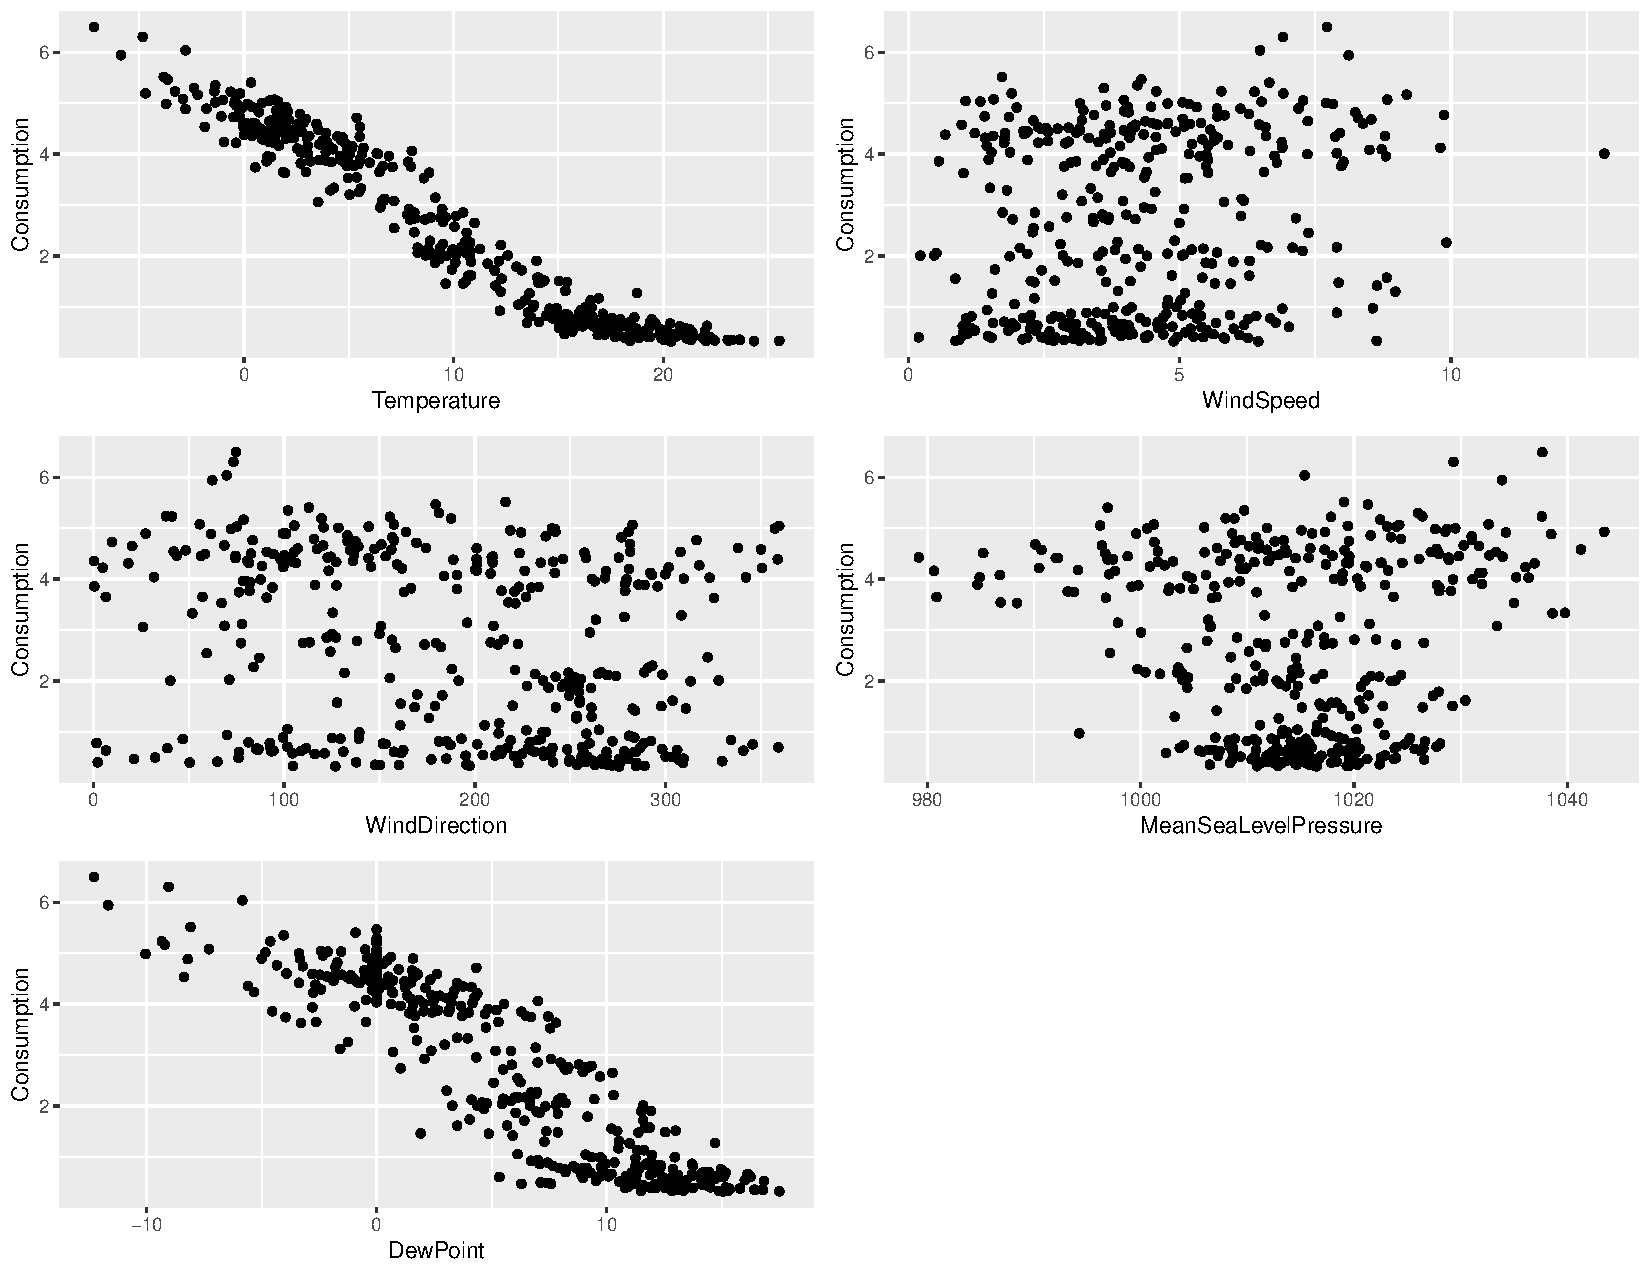
\includegraphics[width=1.\textwidth]{../../../figures/weatherpairs.pdf}
    \caption{Scatterplots of the average consumption for all houses and relevant weather attributes. Each point represents a day. There are clear linearly dependencies between \texttt{Consumption} and \texttt{Temperature}, as was expected}
    \label{fig: weatherpairs}
\end{figure}

\subsection{BBR data}
Presumably, the BBR data has influence on the heat consumption in particular the total area and year of construction. Hence, \cref{fig: bbr_hist} illustrates the house specifications of all houses focusing on the type of house, the total area, the year of construction and reconstruction. 
\begin{figure}
    \centering
    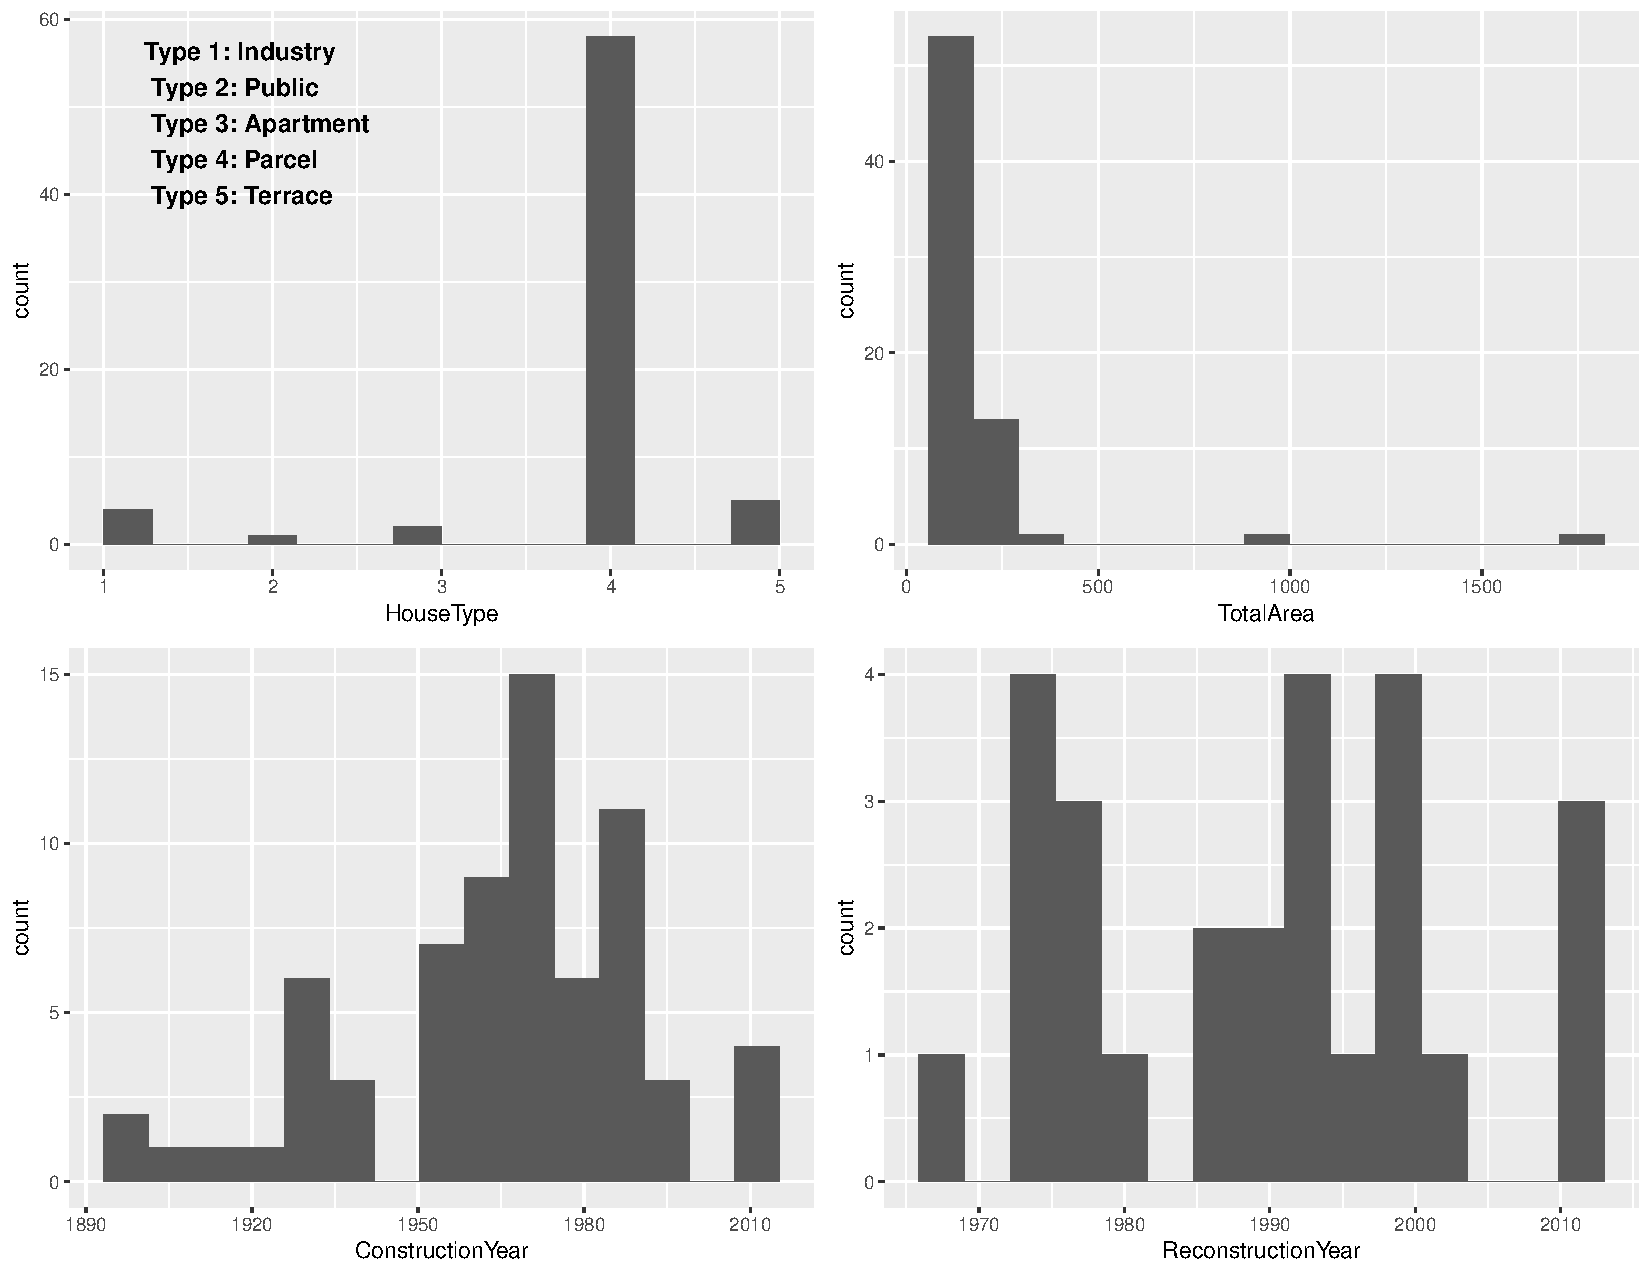
\includegraphics[width=1.\textwidth]{../../../figures/bbr_hist.pdf}
    \caption{Details of the houses from BBR data focusing on the type of house, the total area in $m^2$, the year of construction and reconstruction respectively}
    \label{fig: bbr_hist}
\end{figure}
Since the two houses, 18 and 55, showed in \cref{fig: daily_cons} will be used throughout the report, it is important to know their specifications:
\begin{multicols}{2}
    \begin{itemize}
        \item[]\textbf{House 18:}
        \item House type: Parcel
        \item Area: 128 $m^2$ + attic of 34 $m^2$
        \item Year of construction: 1927
        \item Reconstructed in 1998
    \end{itemize}
    \columnbreak
    \begin{itemize}
        \item[]\textbf{House 55:}
        \item House type: Parcel
        \item Area: 160 $m^2$ 
        \item Year of construction: 1971
        \item Has wood-burning stove 
    \end{itemize}
\end{multicols}
\noindent The areas of the houses are somewhat similar, they are of the same house type and their ages are close to each other. However, house 18 has an odd behaviour which will be evident in the later results. \\

\noindent The average of the heat consumption for each house is found/determined for the winter period. By dividing the average consumption with the total area of the house the consumption pr. $m^2$ is calculated. Figure \ref{fig: byggeaar} shows the year of construction and the consumption for each of the houses. The year of construction is here determined by either the year of construction or the year of the latest reconstruction of a house. 
\begin{figure}
    \centering
    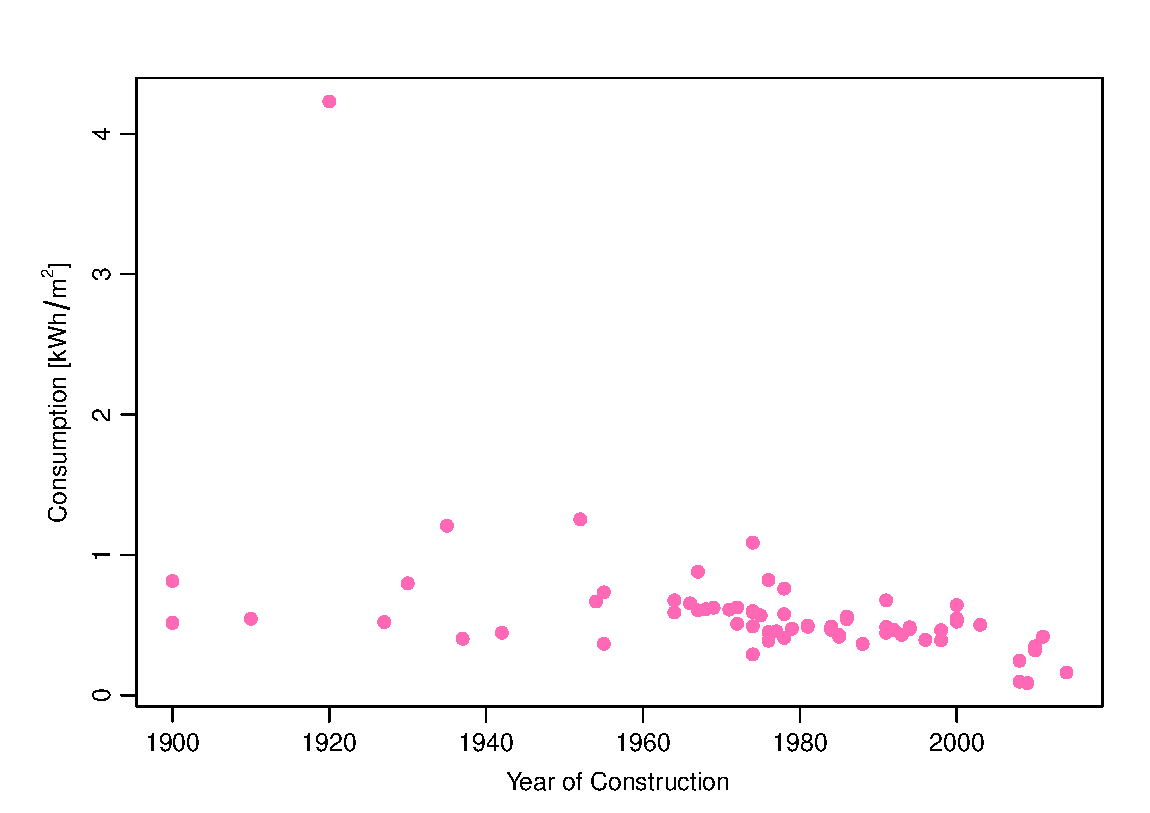
\includegraphics[width=.8\textwidth]{../../../figures/byggeaar.eps}
    \caption{Plot showing the year of construction and the average consumption pr. $m^2$ for each house. It is seen that there is a tendency that the later a house is built or reconstructed, the better is the insulation of the house}
    \label{fig: byggeaar}
\end{figure}

\noindent Figure \ref{fig: byggeaar} shows the relation between the year of construction of a house and its average consumption pr. $m^2$. A single house stands out with a consumption that is remarkably higher than the rest. The house is a simple appartment of $61 m^2$ build in 1920. Other than that, there seems to be a vague tendency that older buildings have a higher consumption. The buildings from after $1990$ all have relatively low consumption, while the older buildings have a higher spread. For houses that have been reconstructed, the reconstruction year has been used instead of the construction year. So some houses in the plot might in fact be older than it is shown here. The nature of the reconstructions is not known, but since they are extensive enough to be registered in BBR, it is assumed to have an effect on the consumption of that house.


\section{Multicollinearity}
Multicollinearity occurs when two or more explanatory variables are highly correlated. In linear regression, multicollinearity \textcolor{red}{\dots} Multicollinearity can be investigated by calculating the correlation using the function \texttt{cor()} in \texttt{R}.\\

\noindent Figure \ref{fig: weather_cons} clearly shows that there is a high correlation between \texttt{Temperature} and \texttt{Dewpoint}. The exact correlation between the two attributes is calculated at 0.936, hence it is decided to remove \texttt{Dewpoint}. Furthermore, it is assumed that \texttt{Radiation} is a replacement for the attributes describing the sun, namely \texttt{Condition} and \texttt{SunHour}. This is the basis for expecting a correlation between the radiation and the sun attributes. Figure \ref{fig: gg_cor} shows a plot of the correlation matrix between the abovementioned attributes.
\begin{figure}
    \centering
    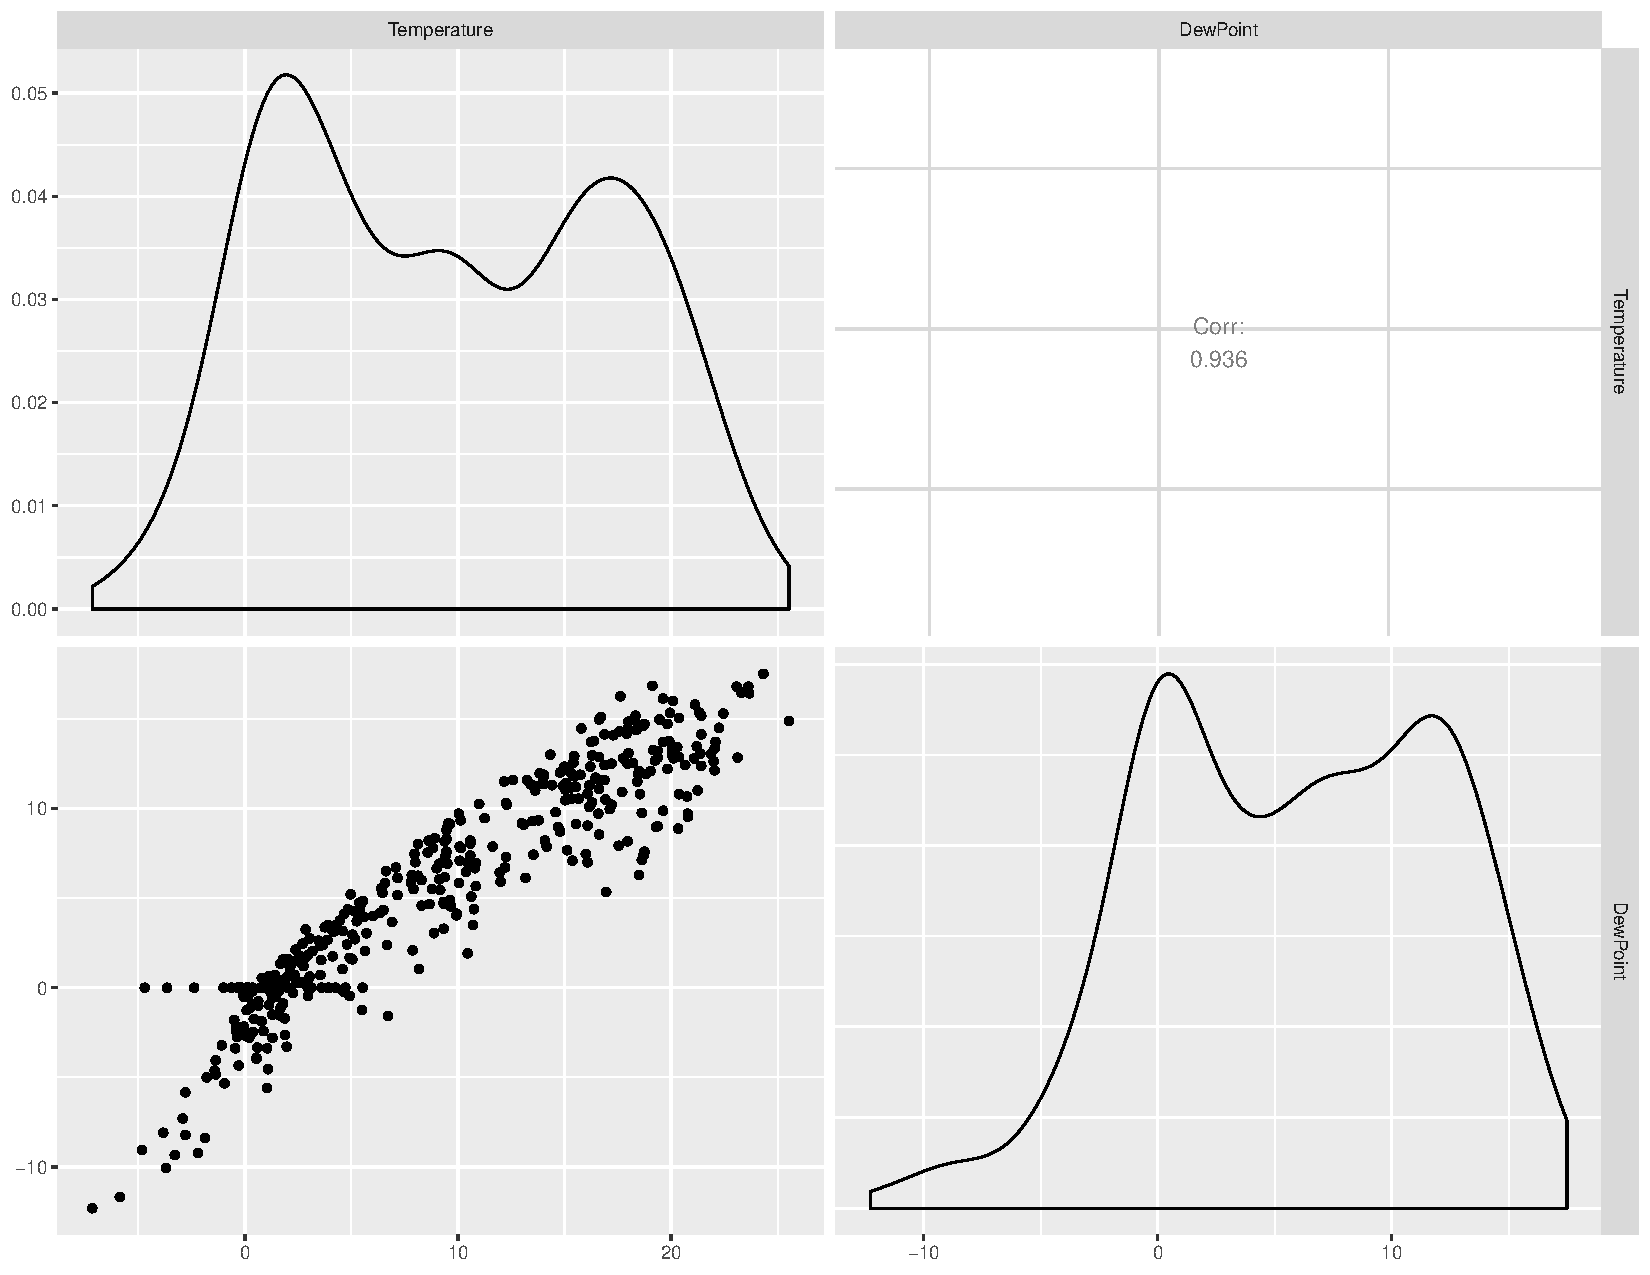
\includegraphics[width=1.\textwidth]{../../../figures/gg_cor.pdf}
    \caption{Scatterplot showing the correlations between the thwo attributes \texttt{Temperature}, \texttt{DewPoint}. It is clearly seen that the temperature and dew point are highly correlated}
    \label{fig: gg_cor}
\end{figure}
\noindent There is a high correlation between \texttt{Radiation} and \texttt{SunHour} at 0.955, thus \texttt{SunHour} is removed from the weather data set. \\
 
\noindent The complete data set used for modelling in chapter 4 can be seen in table \ref{tab: modeldata}.
\begin{table}
    \centering
    \begin{tabular}{ll}
     \hline
     \textbf{Variable} & \textbf{Description} \\
    \hline
    \hline
    Date  &  End time and date for measurements. Hourly values\\
    Temperature  &  Temperature outside in Degrees/C \\
    WindSpeed  &  In $m/s$\\ 
    WindDirection  &  In degrees\\
    Condition  & The condition of the weather given in integers described in \cite{condition}\\
    MeanSeaLevelPressure & Avg. atmospheric pressure at mean sea level in mbar.\\
    PrecipitationProbability & Measure of the probability that precipitation will occur. \\
    Observation & The number of observations for each day for each house.\\
    Consumption & CoolingDegree times Volume from House data \\
    Holiday & A categorical attribute with 6 levels: Working day, \\ & Weekend, Autumn break, Christmas break, \\ & Winter break and Spring break.\\
    \hline
    \end{tabular}
    \caption{Attributes used for modelling}
    \label{tab: modeldata}
\end{table}   

\section{Data segmentation}
All the models used in this project assume that there is a linear relationship between the outside temperature and the heat consumption of a house. It would make sence that the heat consumption of a house increases as the temperature decreases. But this is mostly true when it is actually cold. In the summer time the heat consumption is generally not dependent on the outside temperature. \cref{fig: Consumption-PW} shows two examples of the relationship between temperature and consumption. It can be seen that some houses have a very linear relationship between temperature and consumption, and others less so. Most have in common that for high temperatures, the consumption reaches a more or less constant low level. This relationship most likely shows that when the heating is turned on, the consumption rises and falls with the outside temperature. When the heating is not turned on, the only consumption is the tap water consumption. One of the main challenges of this project is that the data does not provide a simple way of distinguishing between tap water consumption and heating consumption. If the inhabitants are not home for a longer period, there will probably be low consumption, even though it might be cold outside. This does not necessarily mean that the house is well isolated. And if
there is consumption in warm periods, it is likely to be tap water consumption, and not heating.

\noindent To minimize the effect of tap water consumption this section will explore different ways of extracting the period where the consumption is dominated by heating, and not by tap water. This period will be denoted the winter period for obvious reasons. By only applying the regression models described in Chapter \ref{chap: daily} to the period dominated by heating, deviations caused by tap water consumption will hopefully be less significant. If a linear model was used on the entire data, the variation of the relation between temperature and consumption would be far from constant during the year, violating a key assumption of the model. The approach used in this section is to search for a temperature that can be used as a threshold. All days with average temperatures below the threshold will be classified as belonging to the winter period. Two ways of finding this threshold will be described below. Other more sophisticated ways to make the classification of the winter period might be applied, but they will not be considered in this project.


\subsection{Segmentation by piece-wise optimization}
The first approach is to make a linear regression on the data with two segments. A breakpoint
$\alpha$ is found, such that the SSE is as small as possible. The second segment is restricted to
being constant. This way the breakpoint can be used as the threshold seperating the winter period from the rest of the data. This method was tested on every available
house, where a new breakpoint was found for each house.

\noindent Figure \ref{fig: Consumption-PW} shows the regression for two different houses. On house 55 the
line fits rather well with the low-temperature data points, but house 18 behaves differently. Neither breakpoints act as a very good threshold. Both houses show very clearly that the assumption that all points below the breakpoint belong to the period without heating is not accurate. Even though this approach can easily take out a lot of data
where there is clearly no heating, it will in many cases set the breakpoint too high. The "tail" of the period without heating might still be included, causing a bias in the model, and some variation that is not accounted for. The method is also not very robust. Depending on how the points are spread out, the breakpoint is sometimes as high as 20 degrees, which is not desirable.
\begin{figure}
    \centering
    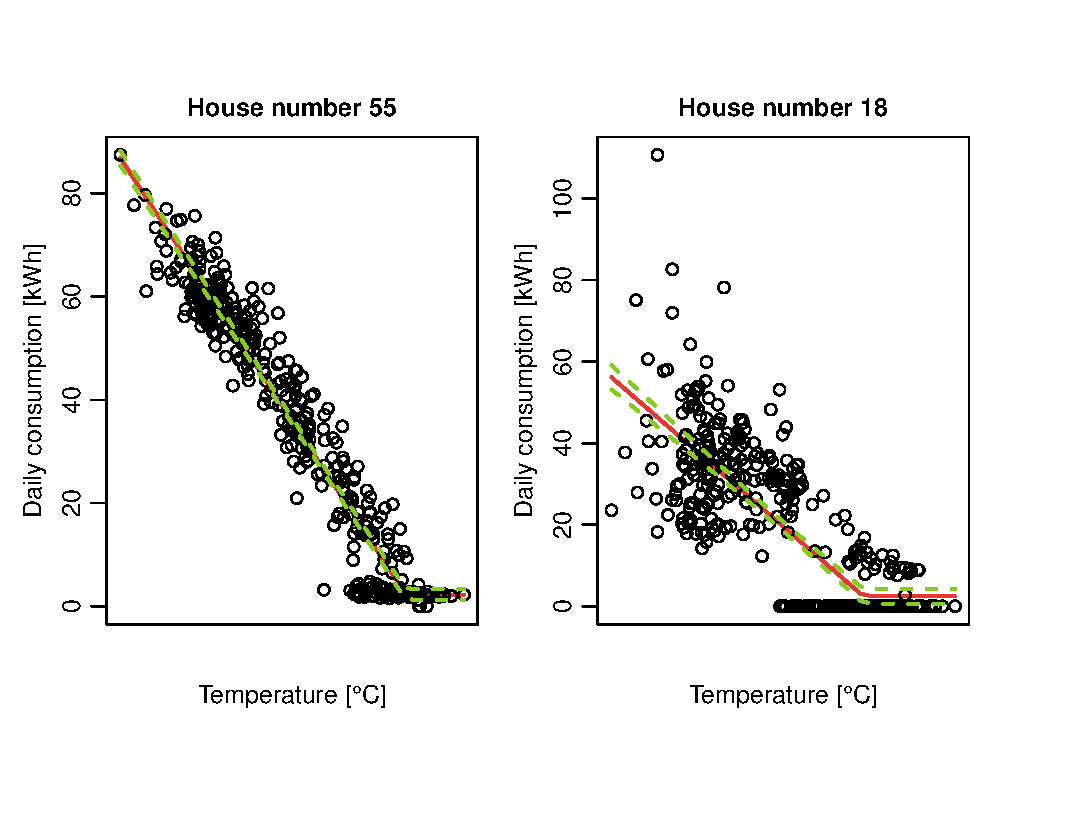
\includegraphics[width=0.8\textwidth]{../../../figures/Consumption_PW.eps}
    \caption{Piece-wise optimization of the consumption. The red line is the regression line and the green line is the confidence interval}
    \label{fig: Consumption-PW}
\end{figure}


\subsection{Segmentation by significant deviations}
In the second approach, all data points with a temperature
above 20 degrees are assumed to belong to the period without heating. Then the mean and standard deviation of a normal distribution containing those points is calculated.
For each degree interval below 20 degrees, if 80\% of the points in that interval are above the confidence interval of the normal distribution, then that degree interval should be included in the winter period. The threshold is set accordingly. \cref{fig: Breakpoint55} shows an example of the procedure on house 55. The left plot shows the confidence interval as a black line. The proportion of the data points above that line is illustrated on the plot on the right. Here the interval between 14 and 15 degrees is the highest where more than 80\% is outside the confidence interval. Thus, 15 degrees is chosen as the threshold. The vertical orange line on the left plot shows this threshold at 15 degrees. This threshold captures almost every point in the beforementioned "tail" with low consumption. A few outliers with very low consumption are still included in the winter period. But overall the classification of the winter period seems to work well for this house. \cref{fig: Breakpoint18} shows the same procedure for house 18. Here the linear dependency between temperature and consumption is not fulfilled very well for any part of the data, but the threshold cuts out the data where there is clearly no consumption at all.

\noindent In general, this model is more robust than the first. It is more selective, and provides a good way to set the threshold on the correct side of the mentioned "tail" that may occur at temperatures both with and without heating.
When comparing \cref{fig: Breakpoint55} and \cref{fig: Breakpoint18} to \cref{fig: Consumption-PW}, one can see that this method sets the breakpoint a bit lower, removing more points without heating. If the consumption data behaves badly, and chunks of datapoints are low enough to be within the confidence interval, then a lot of data can potentially be removed, and there might be too little data left.

Until now the focus has been to find a threshold for every individual house. But the goal is to have a general classification of the winter period. Figure \ref{fig: AlphaHist} shows a histogram of the breakpoint values for every house in the data set. The global breakpoint should be in the low end of the scale. It is better to remove data points that could have been used, than to include too many points that belong to a different distribution with a different variation, which could make the assumptions of the model worse. It would not be good to choose the minimum breakpoint, since that would be very vulnerable. A single house with a very low breakpoint might make the model bad for all the other houses. So the breakpoint that is chosen is the first quantile. As it is shown on the figure, this is 12 degrees. All models in the following sections will only be considering data where the temperature less than or equal to 12 degrees. At some point it will also be of interest to look at the summer period. This will be defined as the data with temperatures above 15, as that is the third quantile in \cref{fig: AlphaHist}. This way there is a temperature gap between the summer and winter period, that is not included in any of them. Out of the total 396 days covered by the house data, 239 are classified as winter days, 126 as summer days, and 31 days are neither summer nor winter days. \cref{fig: class_breakpoint} shows how the days are distributed. It can be seen that the winter days are a continouos period from January to August 2018 and again from November 2019
\begin{figure}
    \centering
    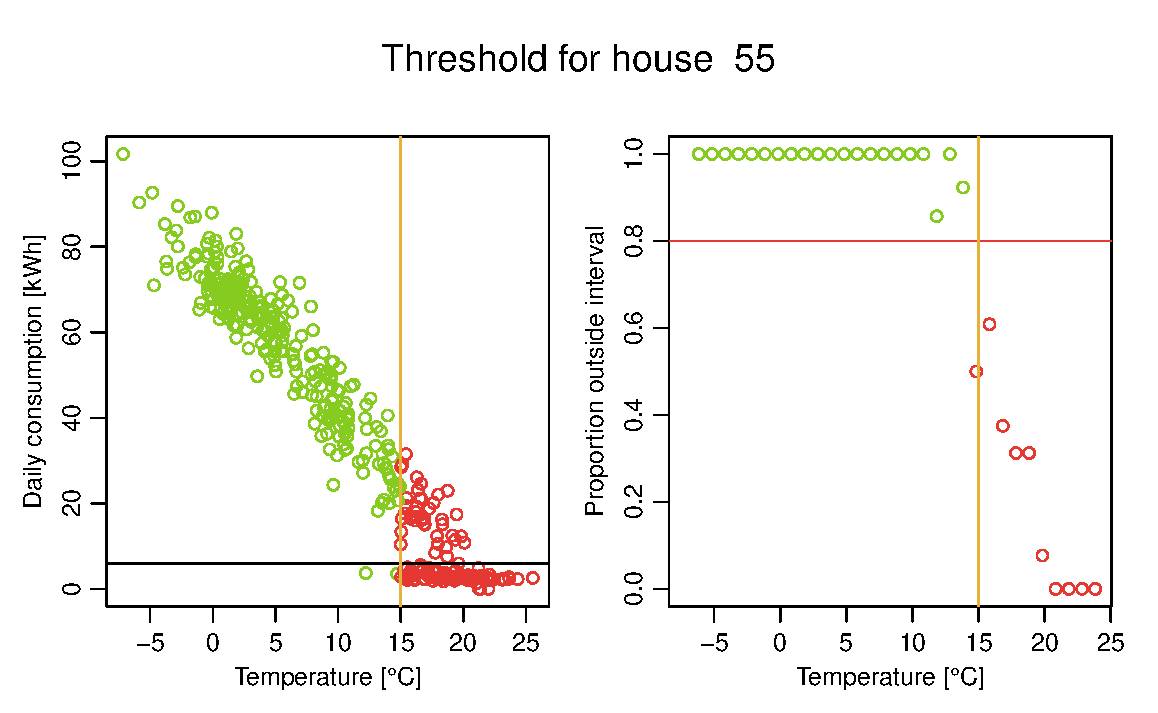
\includegraphics[width=0.8\textwidth]{../../../figures/Breakpoint_55.eps}
    \caption{An illustration of how the breakpoint is found using segmentation by significant deviations. On the left figure the black line illustrates the confidence interval of the normal distribution containing points above 20 degrees. The right figure shows for each degree interval, the proportion of data points that are outside the confidence interval. The last point below 80\% is the chosen breakpoint}
    \label{fig: Breakpoint55}
\end{figure}
\begin{figure}
    \centering
    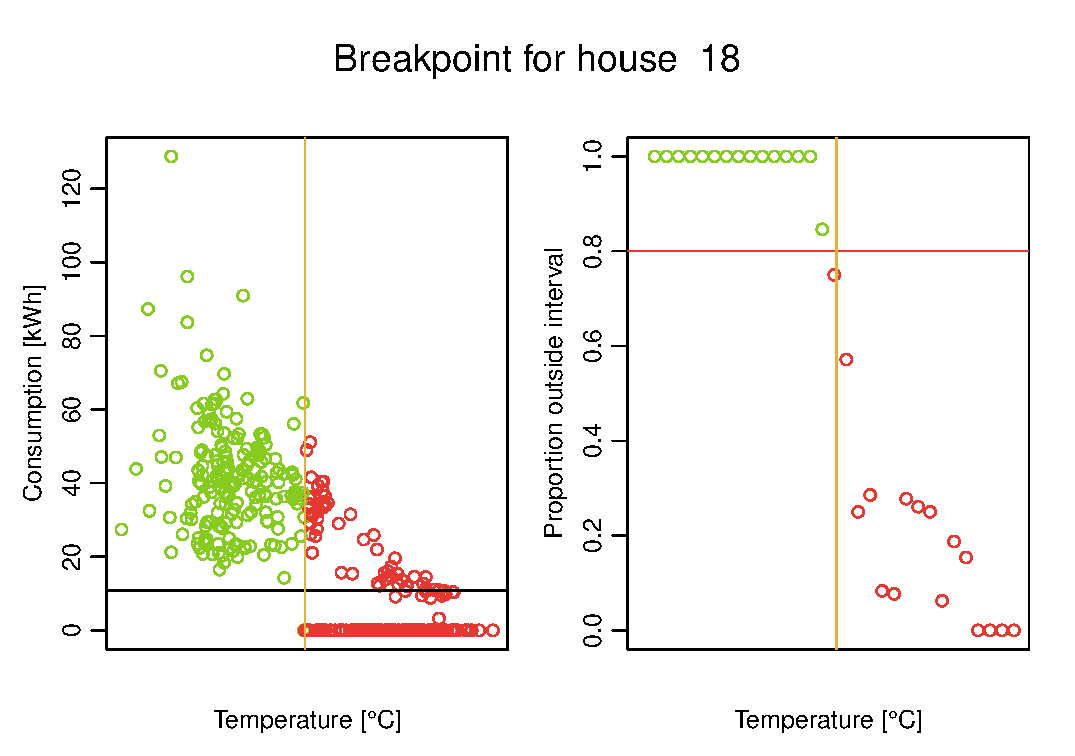
\includegraphics[width=0.8\textwidth]{../../../figures/Breakpoint_18.eps}
    \caption{This figure shows the same as \cref{fig: Breakpoint55}, but for house 18 instead. The assumption of a linear relationship between temperature and consumption is worse for this house}
    \label{fig: Breakpoint18}
\end{figure}
\begin{figure}
    \centering
    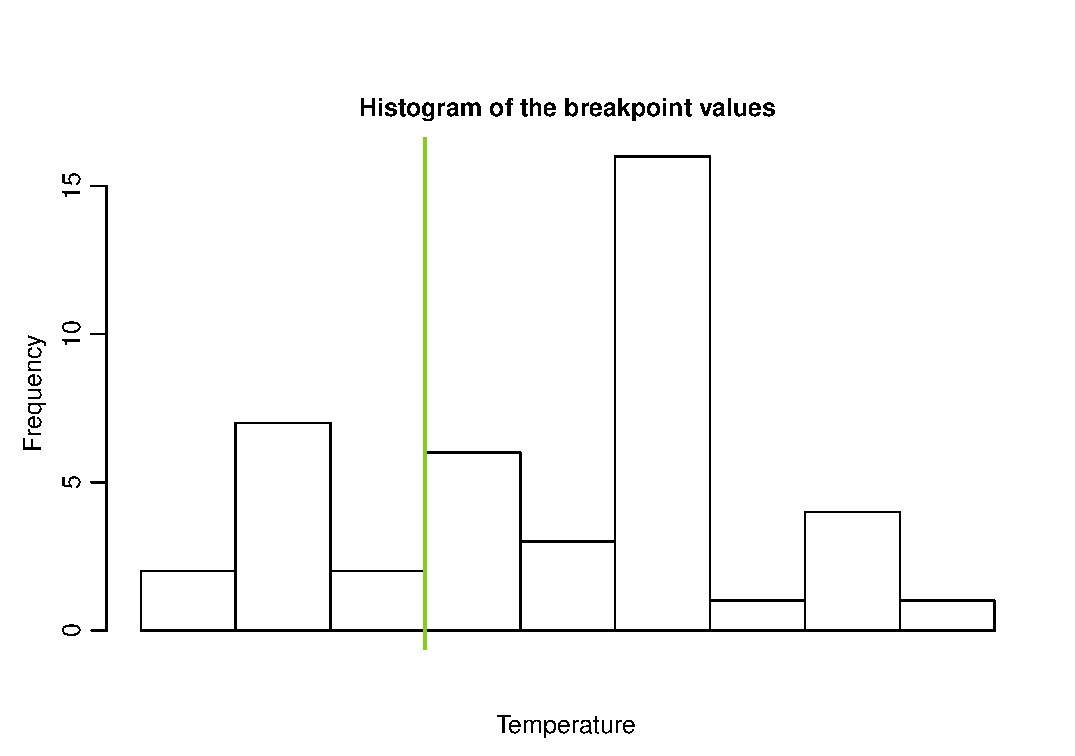
\includegraphics[width=0.8\textwidth]{../../../figures/AlphaHist.eps}
    \caption{A histogram of the alpha values for every house in the third segmentation method. The first quantile is chosen as the overall breakpoint. It is 12 degrees, illustrated by the green line}
    \label{fig: AlphaHist}
\end{figure}

\begin{figure}
    \centering
    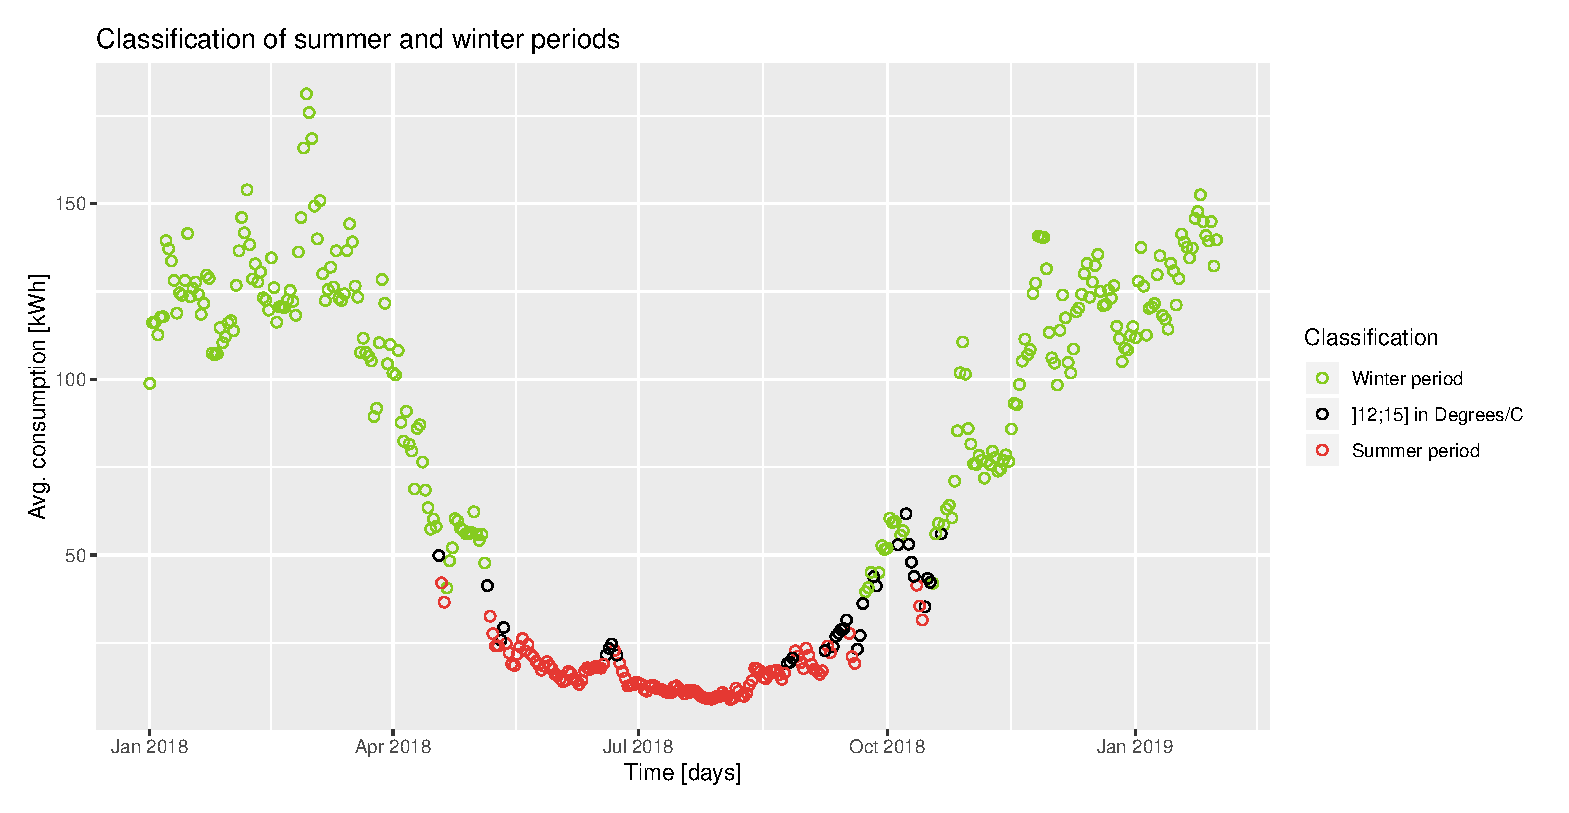
\includegraphics[width=1.\textwidth]{../../../figures/class_breakpoint.eps}
    \caption{The average consumption of all houses, coloured by the period that the day is included in}
    \label{fig: class_breakpoint}
\end{figure}
